\chapter{Cinématique des milieux continus}
\section{Les vitesses de déformation}

\subsection{Vitesse de rotation}
\begin{wrapfigure}[6]{r}{2cm}
	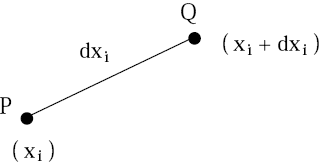
\includegraphics[scale=0.4]{ch3/image1.png}
	\captionof{figure}{Milieu continu}
\end{wrapfigure}
Si je malaxe mon chewing-gum, il se déforme et il faut bien que je puisse le quantifier.
Pour ce faire, considérons deux points voisins $P$ et $Q$ et exprimons la vitesse de $Q$
en fonction de $P$ (développement en série tronqué au premier ordre) : 
\begin{equation}
	v_i(Q) = v_i(P) + \left[
	\dfrac{\partial v_i}{\partial x_j}\right]_P dx_j + \dots = v_i(P) + v_{i,j} dx_j + \dots
\end{equation}
On trouve donc $dv_i = v_i(Q) - v_i(P) = v_{i,j}dx_j$.\\
    
Décomposons le tenseur $v_{i,j}$ en sa partie symétrique et antisymétrique afin d'étudier 
séparément l'interprétation physique de chacune des parties.
\begin{equation}
	v_{i,j} = v_{(i,j)} + v_{[i,j]}\ \ \ \text{où}\ \left\{\begin{array}{lll}
	v_{(i,j)} &=& \frac{1}{2}(v_{i,j}+v_{j,i})\\
	v_{[i,j]} &=& \frac{1}{2}(v_{i,j}-v_{j,i})
	\end{array}\right.
\end{equation}
On notera alors $dv_i = dv_i^* + dv_i^{**}$ (distribution de la partie sym. et antisym.).

\subsubsection{Étude de la partie antisymétrique}
Pour se faire, on va utiliser le vecteur rotationnel en définissant le \textit{vecteur
	tourbillon} : $\vec \omega = \frac{1}{2}\overline{rot}\ \vec{v}$, ou en notation indicielle:
\begin{equation}
	\omega_i = \frac{1}{2}\delta_{ijk}\partial_jv_k
\end{equation}
         
Pour garder la composante antisymétrique introduite par le produit vectoriel, on va
multiplier l'expression du vecteur tourbillon par $\delta_{ipq}$ pour avoir :
\begin{equation}
	\delta_{ipq}\omega_i = \frac{1}{2}\delta_{ipq}\delta_{ijk}\partial_jv_k
\end{equation}
Le produits des $\delta$ avec le premier indice en commun me permet d'écrire ($\delta$
en première position - $\delta$ avec indice croisé) (formule d'expulsion) :
\begin{equation}
	\delta_{ipq}\omega_i = \frac{1}{2}(\delta_{pj}\delta_{qk} - \delta_{pk}\delta_{qj})
	v_{[p,q]}
\end{equation}
Où encore : 
\begin{equation}
	\delta_{ipq}\omega_i = \frac{1}{2}(v_{[q,p]}-v_{[p,q]}) = v_{[q,p]}
\end{equation}
$\Rightarrow$ seule la partie antisymétrique des dérivées de la vitesse intervient.\\
         
Compte tenu de cette expression, on peut ré-écrire notre partie antisymétrique :
\begin{equation}
	dv_i^{**} = v_{[i,j]}dx_j = \delta_{ijk}\omega_jdx_k
\end{equation}
ou, en notation vectorielle : $\overline{dv}^{**} = \overline{\omega}\times
\overline{PQ}$.\\
La partie antisymétrique représente donc un mouvement de rotation de corps indéformable
autour du point $P$. Et la déformabilité ? Elle se cache forcément dans la partie
symétrique.
         
         
         
         
         
\subsubsection{Étude de la partie symétrique}
\begin{wrapfigure}[7]{l}{3.5cm}
	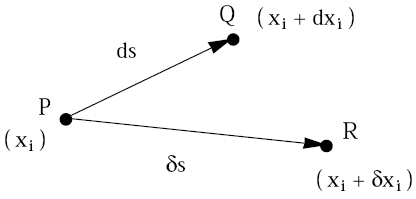
\includegraphics[scale=0.3]{ch3/image2.png}
	\captionof{figure}{Milieu continu}
\end{wrapfigure}
Si j'ai une vitesse d'allongement, je vais avoir déformation.  Considérons deux points
$Q$ et $R$ voisins de $P$ tel que\footnote{Le $\delta$ est là pour éviter les confusions.}
\begin{equation}
	dv_i = v_i(Q) - v_i(P) = v_{i,j} dx_j\ \ \ \ \ \ \ \ \delta v_i = v_i(R) - v_i(P) =
	v_{i,j}\delta x_j
\end{equation}
         
La dérivée du produit scalaire $(ds.\delta s)$ permettra de caractériser celle-ci
\footnote{Ce produit scalaire ne change que si une des longueurs (ou l'angle) change.}. En
effectuant (détails slide 11), on obtient\footnote{Aide pour ceux qui veulent le calculer :
	Les indices étants muets, on peut les permuter pour obtenir $dx_i\delta x_j$ afin de le
mettre en évidence.} :
\begin{equation}
	(dx_i\ \delta x_i)^\bullet = 2v_{(i,j)} dx_i\delta x_j
\end{equation}
         
         
\subsection{Tenseur des vitesses de déformation}
Nous avons ainsi trouvé que $(dx_i\ \delta x_i)^\bullet = 2v_{(i,j)} dx_i\delta x_j$ avec :
\begin{equation}
	V_{ij} = \frac{1}{2}(v_{i,j} + v_{j,i}) = v_{(i,j)}
\end{equation}
$\Rightarrow$ il s'agit d'un tenseur symétrique du second ordre et possède toutes les propriétés
établies pour le tenseur des contraintes (valeurs/directions principales, Mohr, formule analytique
de changements d'axes, ...). Il s'agit d'une fonction linéaire !
    
    
\subsubsection{Signification physique des composantes de $V_{ij}$}
Dérivons le même produit scalaire qu'un peu plus haut, mais formulé de façon différente (bien
entendu équivalente)
\begin{equation}
	(dx_i\ \delta x_i)^\bullet = (\vec{ds}.\vec{\delta s})^\bullet = (ds\ \delta s \ \cos
	\theta)^\bullet
\end{equation}
Après avoir mis en évidence $ds\ \delta s$, je divise par ces termes mis en évidence pour 
obtenir\footnote{'Détails' slide 13.} :
\begin{equation}
	\left[\left( \dfrac{\dot{ds}}{ds}+\dfrac{\dot{\delta s}}{\delta s}\right)\cos\theta - \dot{
		\theta}\sin\theta\right]
\end{equation}
Je trouve alors :\\
        
\prop{
	\begin{equation}
		\left[\left( \dfrac{\dot{ds}}{ds}+\dfrac{\dot{\delta s}}{\delta s}\right)\cos\theta - \dot{
			\theta}\sin\theta\right]= 2 V_{ij}\mu_i\nu_j
	\end{equation}}
       
      
      
      
      
\section{Les déformations}
    
\subsection{Tenseur des déformations de Green}
\begin{wrapfigure}[9]{l}{4.5cm}
	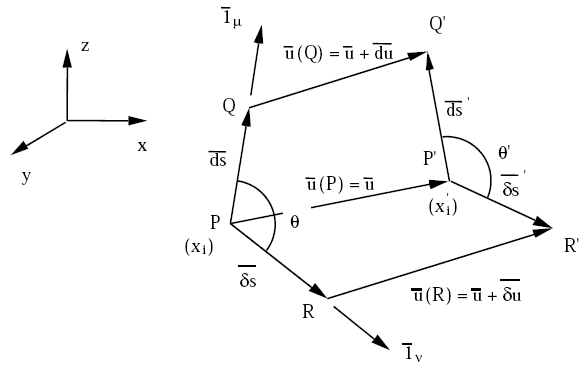
\includegraphics[scale=0.3]{ch3/image3.png}
	\captionof{figure}{Green}
\end{wrapfigure}
Considérons une fois de plus le déplacement d'un point $P$ et de deux points $Q,R$ infiniment
voisins ($u \rightarrow u+du, \theta \rightarrow \theta', \dots$). Evaluons les nouvelles 
cooronnées :
\begin{equation}
	\begin{array}{ll}
		x_i'(Q') & = x_i(Q) + u_i(Q) \\
		x_i'(P') & = x_i(P) + u_i(P) 
	\end{array}
\end{equation}
En soustrayant ces deux équations :
\begin{equation}
	[x_i'(Q') - x_i'(P')] = [x_i(Q)-x_i(P)]+[u_i(Q) - u_i(P)]\ \ \ \equiv dx_i' = dx_i + du_i
\end{equation}
     
Ici je ne vais plus travailler en décomposant la partie symétrique et antisymétrique, mais je 
vais regarder la valeur de mon produit scalaire avant et après :
\begin{equation}
	\overline{ds'}.\overline{\delta s'} - \overline{ds}.\overline{\delta s} = ds'.\delta s'\cos\theta
	- ds. \delta s \cos\theta
\end{equation}
En effectuant ce produit scalaire d'une autre façon, on arrive à : 
\begin{equation}
	\begin{array}{ll}
		\overline{ds'}.\overline{\delta s'} - \overline{ds}.\overline{\delta s} & =dx_i'.\delta x_i' - dx_i.                                                
		\delta x_i\\
		                                                                        & = [dx_i + u_{i,j}dx_j][\delta x_i + u_{i,k} \delta x_k] - dx_i.\delta x_i \\
		                                                                        & = [u_{k,j} + u_{j,k} + u_{i,j}u_{i,k}]dx_j\delta x_k                      \\
		                                                                        & = 2 L_{jk} dx_j \delta x_k                                                
	\end{array}
\end{equation}
Pour arriver à ce résultat, il faut effectuer le double produit de la deuxième équation pour 
ensuite mettre $dx_k\delta x_k$ en évidence (je peux "tripoter" mes indices car ceux-ci sont 
muets, ça n'a pas d'importance). Le crochet de l'avant dernière ligne est nommé $2L_{jk}$, 
soit deux fois le \textit{tenseur des déformations de Green} qui vaut :
\begin{equation}
	L_{jk} = \dfrac{1}{2}\left[\dfrac{\partial u_k}{\partial x_j}+\dfrac{\partial u_j}{\partial x_k}
	+\dfrac{\partial u_i}{\partial x_j}\dfrac{\partial u_i}{\partial x_k}\right]
\end{equation}
Le dernier terme de ce tenseur n'est \textbf{pas} linéaire, si je multiplie $L_{jk}$ par 2,
il serait multiplié par 4. Le caractère non-linéaire fait que l'on n'est pas certain qu'une
solution existe et que si on en trouve une, qu'elle soit unique.\\
Etant un tenseur, on retrouve cependant bien toutes les propriétés associées (Mohr, valeurs
principales, ...)\\
    
En égalant nos deux expressions du produit scalaire et après division par $ds.\delta s$ :
\begin{equation}
	\dfrac{ds'}{ds}.\dfrac{\delta s'}{\delta s}\cos\theta' - \cos\theta = 2L_{jk}\mu_j\nu_k
\end{equation}
    
\subsection{Tenseur des déformations évanouissantes}
Supposons que les dérivées de déplacement sont négligeables devant 1, et que les positions 
avant et après déformations peuvent être confondues : cela permet de négliger le dernier 
terme du tenseur de Green et que $L_{jk}$ devienne une fonction linéaire des déplacements:
\begin{equation}
	a_{jk} = \frac{1}{2}\left[\dfrac{\partial u_k}{\partial x_j}+
	\dfrac{\partial u_j}{\partial x_k}\right]
\end{equation}
Souvent, $a_{ij} (= u_{(i,j)})$ est appelé $\epsilon_{ij}$. Le facteur deux trouvera son 
interprétation plus tard. Pour s'y retrouver, on utilisera $\epsilon$ dans la diagonale et
$\gamma$ hors de celle-ci (\textbf{attention} au facteur 1/2!) :
\begin{equation}
	\left[\begin{array}{ccc}
		\epsilon_x & \dfrac{1}{2}\gamma_{xy} & \dfrac{1}{2}\gamma_{xz}\\
		\dfrac{1}{2}\gamma_{xy} & \epsilon_{y} & \dfrac{1}{2}\gamma_{yz}\\
		\dfrac{1}{2}\gamma_{xz} & \dfrac{1}{2}\gamma_{yz} & \epsilon_{z}
	\end{array}\right]
\end{equation}
    
\subsubsection{Signification physique des composantes de $a_{ij}$}
Considérons que les deux vecteurs soient orientés selon la direction $\vec{1_x}$
\begin{center}
	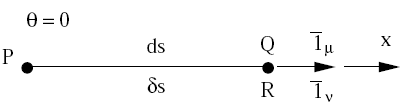
\includegraphics[scale=0.5]{ch3/image4.png}
	\captionof{figure}{Vecteurs alignés selon l'axe $x$}
\end{center}
        
En appliquant $\dfrac{ds'}{ds}.\dfrac{\delta s'}{\delta s}\cos\theta' - \cos\theta
= 2a_{jk}\mu_j\nu_k$ (où $\theta = 0$ comme $Q=R$ et $\mu_i = \nu_i = (1,0,0)$) :
\begin{equation}
	\left(\dfrac{dx'}{dx}\right)^2 - 1 = 2a_{xx}
\end{equation}
Ce qui donne :
\begin{equation}
	1 + 2a_{xx} = \left(\dfrac{dx'}{dx}\right)^2 = \left(\dfrac{dx'-dx}{dx}+1\right)^2
	= \delta_x^2 + 2\delta_x + 1
\end{equation}
L'\textit{allongement relatif dans la direction $x$} est alors donné par 
\begin{equation}
	a_{xx} = \dfrac{dx'-dx}{dx} = \delta_x
\end{equation}
        
\begin{wrapfigure}[9]{r}{3cm}
	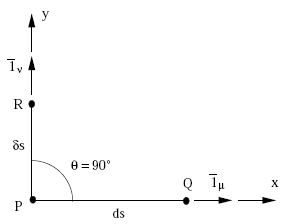
\includegraphics[scale=0.5]{ch3/image5.png}
	\captionof{figure}{Direction $\perp$}
\end{wrapfigure}
Considérons maintenant comme direction $\mu_i = (1,0,0)$ et $\nu_i=(0,1,0)$, avec donc 
un angle de $90\ \deg$. En appliquant notre égalité ci-dessus, on a cette fois 
\begin{equation}
	\dfrac{dx'}{dx}.\dfrac{\delta y'}{\delta y}\cos\theta' = 2a_{xy}
\end{equation}
\textit{"Je vous fais grâce des calculs (à faire chez soi après avoir pris une aspirine
)"}. On trouve dès lors :
\begin{equation}
	2a_{xy} = -\delta_\theta
\end{equation}
ce qui montre une diminution de l'angle initialement droit entre $x$ et $y$. 
        
        
\subsubsection{Les unités du tenseur des déformations}
La composante $\epsilon_x = \partial u/\partial x$, soit une longueur sur une longueur.
Le tenseur des déformations est donc dimensionnel, souvent de l'ordre du micron. On 
introduit ainsi l'unité adimensionnelle, le \textit{microstain} (stain voulant dire
déformation)
\begin{equation}
	1\mu S \equiv 10^{-6}
\end{equation}
